\documentclass[crop,tikz,12pt,border=1pt]{standalone}

\usepackage{tikz}
% \usetikzlibrary{matrix}
% \usetikzlibrary{arrows.meta}
\usetikzlibrary{calc}
% \usetikzlibrary{fit}
\usetikzlibrary{decorations.pathreplacing}
\usetikzlibrary{positioning}

\definecolor{bg1}{RGB}{244,231,195}
\definecolor{bg2}{RGB}{234,204,161}
\definecolor{l1}{RGB}{209,148,106}

\begin{document}

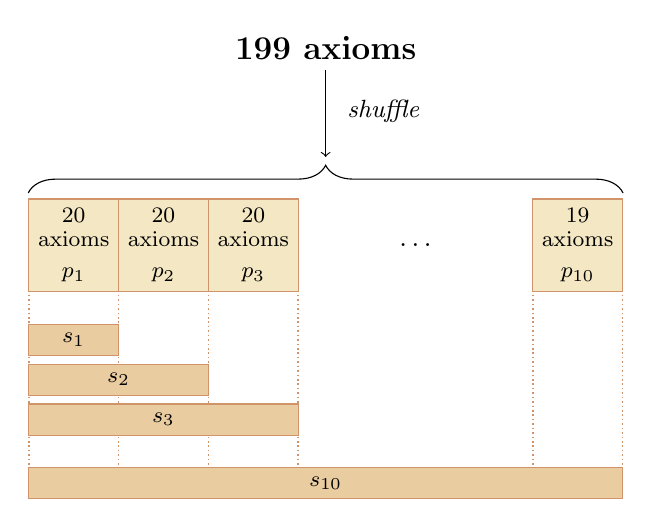
\begin{tikzpicture} [
    p/.style={
        font=\footnotesize,
        align=center,
        draw=l1, fill=bg1
    },
    s/.style={
        font=\footnotesize,
        draw=l1, fill=bg2,
        anchor=west
    },
    dd/.style={
        densely dotted,color=l1, line width=0.6pt,
        transform canvas={xshift=-0.2pt,yshift=-1pt}
    }
]

\pgfdeclarelayer{background}
\pgfsetlayers{background,main}

\node [font=\large\bfseries] (199) {199 axioms};
\node [p] (p1) at (-3.2, -2.5)            {20\\[-0.2ex]axioms\\[0.5ex]$p_1$};
\node [p,right=-\pgflinewidth of p1] (p2) {20\\[-0.2ex]axioms\\[0.5ex]$p_2$};
\node [p,right=-\pgflinewidth of p2] (p3) {20\\[-0.2ex]axioms\\[0.5ex]$p_3$};
\node [p] (p10) at (3.2, -2.5)            {19\\[-0.2ex]axioms\\[0.5ex]$p_{10}$};

\draw [decorate,decoration={brace,amplitude=10pt},rotate=270]
    ($(p1.north west) + (-2pt, 0)$) -- ($(p10.north east) + (-2pt, 0)$);

\draw [->] (199) -- ++ ($(0, 0 |- p10.north) + (0, 15pt)$);
\node [anchor=west,xshift=1ex,font=\small\itshape] at (0, -0.8) {shuffle};

\node at ($(p3)!0.5!(p10)$) {\ldots\unkern};

% \node [s,below=1cm of p1] (s1) {$s_1$};

\path let \p1 = (p1.south west), \p2 = (p1.north east) in
    node [s,minimum width=\x2-\x1-\pgflinewidth,below=4ex of p1.south west,right] (s1) {$s_1$};

\path let \p1 = (p1.south west), \p2 = (p2.north east) in
    node [s,minimum width=\x2-\x1-\pgflinewidth,below=2ex of s1.south west,right] (s2) {$s_2$};

\path let \p1 = (p1.south west), \p2 = (p3.north east) in
    node [s,minimum width=\x2-\x1-\pgflinewidth,below=2ex of s2.south west,right] (s3) {$s_3$};

\path let \p1 = (p1.south west), \p2 = (p10.north east) in
    node [s,minimum width=\x2-\x1-\pgflinewidth,below=4ex of s3.south west,right] (s10) {$s_{10}$};

\begin{pgfonlayer}{background}

\path (p1.south west)  edge [dd,transform canvas={xshift=0.4pt}] (s10.north west);
\path (p1.south east)  edge [dd] (s1.north east |- s10.north east);
\path (p2.south east)  edge [dd] (s2.north east |- s10.north east);
\path (p3.south east)  edge [dd] (s3.north east |- s10.north east);
\path (p10.south east) edge [dd] (s10.north east);
\path (p10.south west) edge [dd,transform canvas={xshift=0.4pt}] (p10.south west |- s10.north east);

\end{pgfonlayer}

% \matrix (table) [
%     matrix of nodes,
%     row sep=-\pgflinewidth,
%     column sep=-\pgflinewidth,
%     row 2/.style={font=\sffamily,nodes={fill=bg1}},
%     column 2/.style={font=\sffamily,nodes={fill=bg1}},
%     nodes={
%         align=center, minimum size=1cm,
%         text depth=0.5ex,text height=2ex,
%         text width=2em,
%         draw=l1
%     },
%     ndf/.style={draw=none, fill=none}
% ]{
%     \node [ndf] (t11) {}; &
%     \node [ndf] (t12) {}; &
%     \node [ndf] (t13) {}; &
%     \node [ndf] (t14) {}; &
%     \node [ndf] (t15) {}; &
%     \node [ndf] (t16) {}; \\
%     %
%     \node [ndf] (t21) {}; &
%     \node [ndf] (t22) {}; &
%     \node       (t23) {Q}; &
%     \node       (t24) {R}; &
%     \node       (t25) {S}; &
%     \node       (t26) {T}; \\
%     %
%     \node [ndf] (t31) {}; &
%     \node       (t32) {O}; &
%     \node       (t33) {0.40}; &
%     \node       (t34) {0.20}; &
%     \node       (t35) {0.00}; &
%     \node       (t36) {0.00}; \\
%     %
%     \node [ndf] (t41) {}; &
%     \node       (t42) {P}; &
%     \node       (t43) {0.40}; &
%     \node       (t44) {0.20}; &
%     \node       (t45) {0.00}; &
%     \node       (t46) {0.00}; \\
%     %
%     \node [ndf] (t51) {}; &
%     \node       (t52) {R}; &
%     \node       (t53) {0.20}; &
%     \node       (t54) {1.00}; &
%     \node       (t55) {0.46}; &
%     \node       (t56) {0.27}; \\
% };

% \node [fit={($(t31.north west)+(1ex,0)$)(t51.south east)},headerb](e1header){};
% \node [xshift=-1pt,anchor=center,rotate=90] at (e1header.center)
%     {$e$ annotations};

% \node [fit={($(t13.north west)-(0,1ex)$)(t16.south east)},headerb](e2header){};
% \node [yshift=1pt,anchor=center] at (e2header.center) {$e'$ annotations};

% \draw [f] (t53.south) -- ++(0,-10pt) node [font=\bfseries,anchor=north] {0.40};
% \draw [f] (t54.south) -- ++(0,-10pt) node [font=\bfseries,anchor=north] {1.00};
% \draw [f] (t55.south) -- ++(0,-10pt) node [font=\bfseries,anchor=north] {0.46};
% \draw [f] (t56.south) -- ++(0,-10pt) node [font=\bfseries,anchor=north] {0.27};

% \draw [f] (t36.east) -- ++(10pt,0) node [font=\bfseries,anchor=west] {0.40};
% \draw [f] (t46.east) -- ++(10pt,0) node [font=\bfseries,anchor=west] {0.40};
% \draw [f] (t56.east) -- ++(10pt,0) node [font=\bfseries,anchor=west] {1.00};

\end{tikzpicture}

\end{document}
